
\chapter{Instrukcja użytkownika}
\section{Początki pracy  z narzędziem}
Narzędzie pozwala na wygenerowanie formularza Google Forms zakodowanego w formacie JSON, automatyczne generowanie zdjęć na podstawie wstawek w latex'u oraz zarządzanie informacjami o tym, czy dany formularz przyjmuje przesyłane odpowiedzi. Na początek należy jednak pobrać i zainstalować zależności wykorzystywane w pracy.
\subsection{Instalacja}
Na początku należy sklonować \href{https://github.com/agnpawicka/pracaInzynierska/}{repozytorium projektu}.\\
Następnie wejść w folder \textbf{source} oraz uruchomić plik o nazwie ,,install.sh''. Pozwoli to na zainstalowanie potrzebnych bibliotek.
\subsection{Uruchomienie}
Aby uruchomić narzędzie należy uruhomić plik o nazwie ,,run.sh''. Uruchomi on lokalny serwer Node.js'owy oraz stronę internetową z interfejsem użytkownika.
\section{Schemat pliku kodującego (JSON)}

\section{Obsługa narzędzia}
Po uruchomieniu użytkownik widzi stronę w przeglądarce, jak na zdjęciu poniżej:
\begin{figure}
  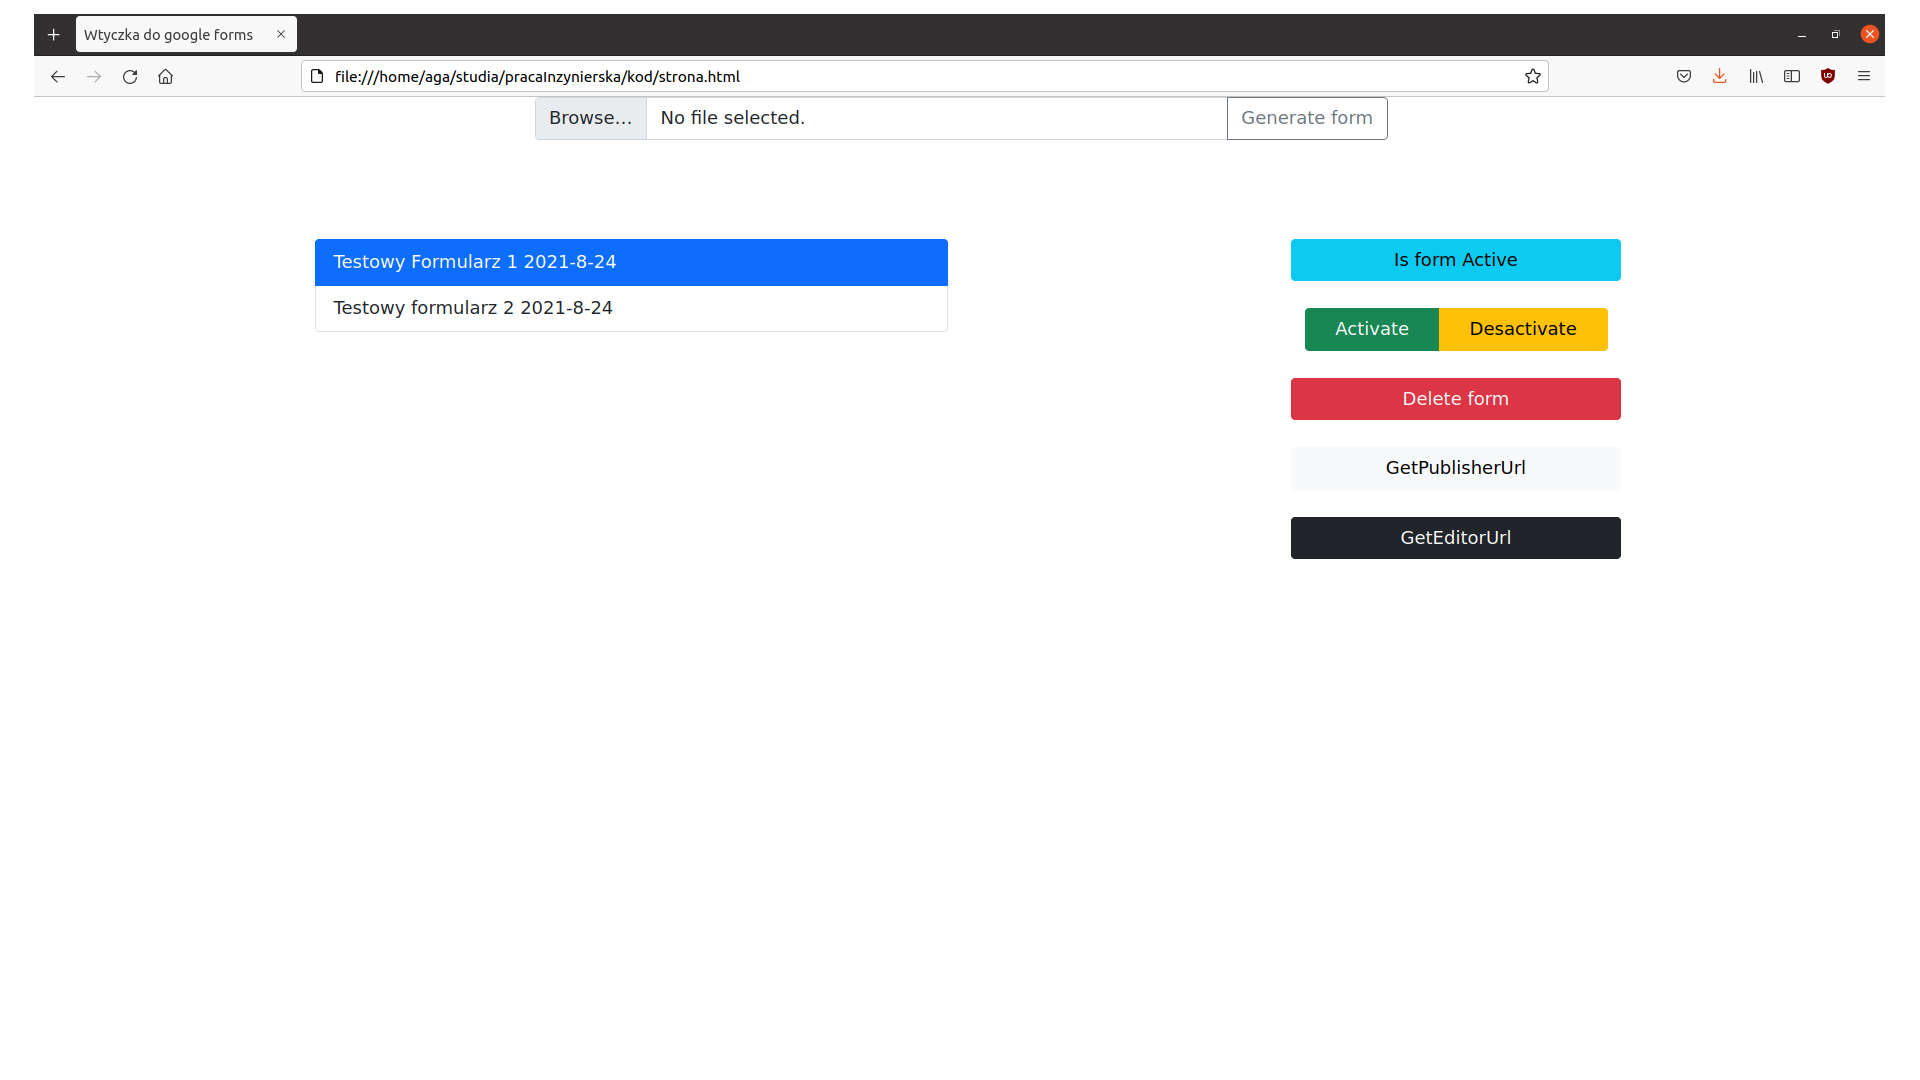
\includegraphics{strona.png}
  \caption{Interfejs aplikacji}
  \label{fig:1}
\end{figure}
\\Widoczne u góry pole do wgrywania plików przyjmuje formaty .txt oraz .json. W pliku powinien znajdować się zakodowany formularz (podrozdział 4.2. Schemat pliku kodującego (JSON)).
\\Poniżej  po lewej stronie znajduje się lista utworzonych już formularzy, po prawej znajdują się przyciski służące do operowania na już istniejących formularzach.
\\Przycisk ,,Generate form'' wgrywa podany plik wykonuje na nim kolejne operacje. Poprawne wykonanie powinno przechodzić przez kolejne etapy:
\begin{itemize}
\item Sprawdzany jest format -  pliku. Jeśli zawartość jest obiektem typu JSON, dane przekazywane są do lokalnego serwera, w przeciwnym przypadku strona wyświetli alert informujący o niepoprawnym formacie.
\item Serwer lokalny sprawdza zgodność pliku ze schematem (JSON schema). Po tym etapie poniżej pola do wgrywania plików powinna pojawić się jedna z poniższych informacji:
\begin{itemize}
\item Validation succeded
\item Wrong JSON format
\end{itemize}
\item Jeśli JSON jest zgodny ze schematem, następuje konwertowanie pytań zakodowanych jako ,,tex'' na format zdjęciowy. 
\item Po zakończonej konwersji z lokalnego serwera wysyłany jest POST request do serwera po stronie Google, gdzie trwa konwersja pliku na formularz. Zdalny serwer odsyła informację po zakończonej pracy do serwera lokalnego.
\item Lokalny serwer dodaje nowy formularz do listy formularzy.
\item Wyświetla się komunikat \textbf{New form has beed created. Please reload page} z prośbą o odświeżenie strony.
\end{itemize}
\\Zachowania poszczególnych przycisków  - za wyjątkiem ,,Generate Form'' - dotyczą zawsze wybranego formularza z listy (podświetlonego w danym momencie na niebiesko). Aby wybrać formularz należy kliknąć na niego w liście formularzy. 
\paragraph{Is Form Ative} przycisk zwraca wartość \textbf{Form is active} jeśli formularz przyjmuje odpowiedzi oraz \textbf{Form is inactive} w przeciwnym przypadku.
\paragraph{Activate} Wysyła do serwera po stornie Google'a zapytanie, jeśli aktywacja formularza przebiegła pomyślnie, zwracana jest wiadomość \textbf{Form activated}.
\paragraph{Deactivate} Wysyła do serwera po stornie Google'a zapytanie, jeśli dezaktywacja formularza przebiegła pomyślnie, zwracana jest wiadomość \textbf{Form deactivated}.
\paragraph{Delete Form} Wysyła do serwera po stronie Google'a zapytanie o dezaktywnację formularza, następnie usuwa z pliku z danymi o formularzach wpis dotczący wybranego formularza oraz w komunikacie \textbf{Form deactivated, please reload page.} prosi o odświeżenie strony
\paragraph{Get Publisher Url} Wysyła do serwera po stronie Google'a zapytanie o adres url dla respondentów wybranego formularza. W komunikacie pojawia się odpowiedni link.
\paragraph{Get Editor Url} Wysyła do serwera po stronie Google'a zapytanie o adres url dla edytorów wybranego formularza. W komunikacie pojawia się odpowiedni link.


